\begin{frame}
    \frametitle{\problemtitle}

    \begin{itemize}
        \item Given are $1 \leq n \leq 10^3$ fences (line segments, $\left|x\right|,\left|y\right|\leq10^6$).
        \item A man lives in each resulting region.
        \item The unbounded region is the ocean.
        \item The distance from a region to the ocean is the number of
        regions to cross to get there.
        \item Crossing through fenceposts or intersection points is not possible.
        \item Are there two neighbouring regions at the same distance
        from the ocean?
    \end{itemize}

    \vspace{1em}
    \centering
    \hfill
    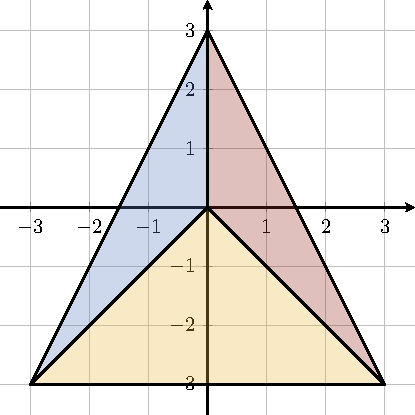
\includegraphics[height=2.5cm]{sample1.pdf}
    \hfill
    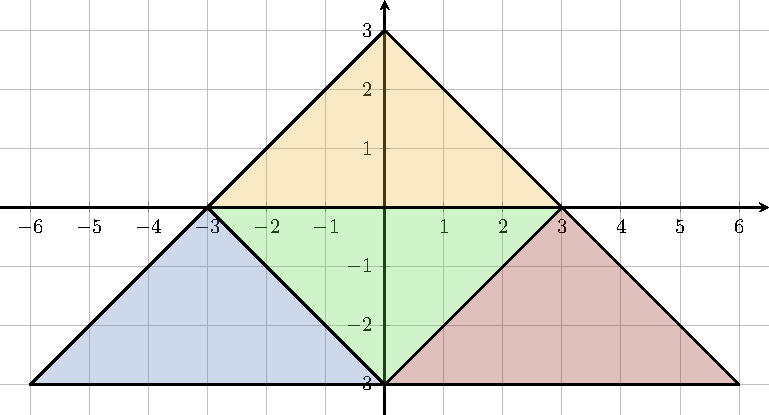
\includegraphics[height=2.5cm]{sample2.pdf}
    \hfill
    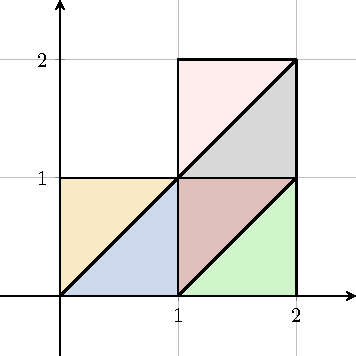
\includegraphics[height=2.5cm]{sample3.pdf}
    \hfill

    \small
    Illustrations of the samples.
    In Sample Input 1 (left), every man has direct access to the ocean. \\
    In Sample Input 2 (middle), no pair of neighbours has the same distance to the ocean. \\
    In Sample Input 3 (right), some pairs of neighbours have the same distance to the ocean
    (e.g., on the left).
\end{frame}
